%!TEX TS-program = pdflatex
% dissertation.tex -- main dissertation file
%
% Wisconsin dissertation template
% Copyright (c) 2008-2009 William C. Benton.  All rights reserved.
%
% This program can redistributed and/or modified under the terms
% of the LaTeX Project Public License Distributed from CTAN
% archives in directory macros/latex/base/lppl.txt; either
% version 1 of the License, or (at your option) any later version.
%
% This program includes other software that is licensed under the
% terms of the LPPL and the Perl Artistic License; see README for details.
%
% You, the user, still hold the copyright to any document you produce
% with this software (like your dissertation).
%

%%% You'll want ``oneside'' for the deposit version, but probably not for any versions that don't need to meet the UW requirements
\documentclass[12pt,oneside,letterpaper]{memoir}

% preamble.tex -- packages to include
%
% Wisconsin dissertation template
% Copyright (c) 2008 William C. Benton.  All rights reserved.
%
% This program can redistributed and/or modified under the terms
% of the LaTeX Project Public License Distributed from CTAN
% archives in directory macros/latex/base/lppl.txt; either
% version 1 of the License, or (at your option) any later version.
%
% This program includes other software that is licensed under the
% terms of the LPPL and the Perl Artistic License; see README for details.
%
% You, the user, still hold the copyright to any document you produce
% with this software (like your dissertation).
\usepackage{float}
\usepackage[section]{placeins}
%% You should use natbib
%\
%\IfFileExists{natbib.sty}{%
%\usepackage[sectionbib]{natbib}%
%\usepackage{chapterbib}
%}{}
\usepackage[backend=biber, style=phys]{biblatex}
\bibliography{thesis.bib}
%% You probably need appendix, if you want appendices
\IfFileExists{appendix.sty}{%
\usepackage{appendix}%
}{}

\usepackage{CJKutf8}

%set table of content and numbering depth
\setcounter{tocdepth}{2}
\setcounter{secnumdepth}{3}

%% the spacing in memoir is weird, you'll need to use this
\DisemulatePackage{setspace}
%\usepackage[doublespacing]{setspace}
\usepackage{setspace}

%% geometry package to help with margins on title page
\usepackage{geometry}

%% List setup; the ``hanglist`` environment will allow you to have
%% nicely-typeset enumerated lists (i.e. with the numbers hanging in
%% the margins).  You need at least version 2.1 of enumitem.sty.  If
%% you don't have enumitem installed at all, hanglist will just be an
%% alias for enumerate.
\IfFileExists{enumitem.sty}{%
\usepackage[loadonly]{enumitem}[2007/06/30]%
\newlist{hanglist}{enumerate}{1}% 
\setlist[hanglist]{label=\arabic*.}%
\setlist[hanglist,1]{leftmargin=0pt}%
}{%
\newenvironment{hanglist}{\begin{enumerate}}{\end{enumerate}}%
}

%% Comment out any of these that you don't want
\usepackage{amssymb}
\usepackage{amsmath}
\usepackage{amsthm}
%\usepackage{theorem}
\usepackage{hyperref}

\IfFileExists{mathpartir.sty}{%
\usepackage{mathpartir}%
}{}

%%%%% LISTINGS package and setup
\IfFileExists{listings.sty}{%
\usepackage{listings}%
}{}



%% Get rid of ugly borders around PDF hyperlinks (e.g. for cross-references, bib entries, or URLs)
\hypersetup{pdfborder = 0 0 0}

%% You want microtype.
\IfFileExists{microtype.sty}{%
\usepackage[protrusion=true,expansion=true]{microtype}%
}{}

%\pagestyle{thesisdraft}

% Surround parts of graphics with box
\usepackage{boxedminipage}

%% booktabs (thx to Nate Rosenblum for bringing this beautiful package
%% to my attention)
\IfFileExists{booktabs.sty}{%
\usepackage{booktabs}%
}{}

% This is now the recommended way for checking for PDFLaTeX:
\usepackage{ifpdf}

%% Avoid ugly "Type 3" fonts
\usepackage{lmodern}
\usepackage[LY1]{fontenc}

%% Substitute your favorite serif and sans fonts here....
\IfFileExists{tgpagella.sty}{%
% TeX Gyre pagella, like Palatino
\usepackage{tgpagella}%
}{}

\usepackage[LY1]{eulervm}

\ifpdf
\usepackage[pdftex]{graphicx}
\else
\usepackage{graphicx}
\fi

\usepackage{makeidx}
\makeindex

{\theoremstyle{plain}
\newtheorem{thm}{Theorem}[chapter]
\newtheorem{cor}[thm]{Corollary}
\newtheorem{define}[thm]{Definition}
\newtheorem{exmpl}[thm]{Example}
}
{\theoremstyle{remark}
\newtheorem{rmk}[thm]{Remark}
}

\newtheoremstyle{customsty1}
{3pt}%
{3pt}%
{}% --- body font
{}% --- indent amount
{\bfseries}% --- Theorem head font
{:}% --- Punctuation after head
{.5em}% --- space after head
{}% --- theorem head spec (can be left empty, meaning 'normal')

% Define 'newtheorems' that use ``customsty1''
{\theoremstyle{customsty1} 
}


%%% NB: the ``deposit'' chapter- and page- styles should conform to UW
%%% requirements.  If you are producing a pretty version of your
%%% dissertation for web use later, you will certainly want to make
%%% your own chapter and page styles.

\makechapterstyle{deposit}{%
  \renewcommand{\chapterheadstart}{}
  \renewcommand{\printchaptername}{}
  \renewcommand{\chapternamenum}{}
  \renewcommand{\printchapternum}{\parbox{2em}{\MakeLowercase{\Large\scshape\thechapter{}}} }
  \renewcommand{\afterchapternum}{}
  \renewcommand{\printchaptertitle}[1]{%
  \raggedright\Large\scshape\MakeLowercase{##1}}
  \renewcommand{\afterchaptertitle}{%
  \vskip\onelineskip \hrule\vskip\onelineskip}
}

\makepagestyle{deposit}
 
\makeatletter
 
\renewcommand{\chaptermark}[1]{\markboth{#1}{}}
\renewcommand{\sectionmark}[1]{\markboth{#1}{}}
 
\makeevenfoot{deposit}{}{}{}
\makeoddfoot{deposit}{}{}{}
\makeevenhead{deposit}{\thepage}{}{}
\makeoddhead{deposit}{}{}{\thepage}
\makeatother

%%% set up page numbering for chapter pages to satisfy UW requirements
%%% NB: You will want to delete until the ``SNIP'' mark if you are
%%% making a ``nice'' copy
\copypagestyle{chapter}{plain}
\makeoddfoot{chapter}{}{}{}
\makeevenhead{chapter}{\thepage}{}{}
\makeoddhead{chapter}{}{}{\thepage}
%%% SNIP

%%% bib nonsense
\makeatletter
\newenvironment{wb-bib}[1]{%
  \chapter*{references}
\ifnobibintoc\else 
\phantomsection 
%\addcontentsline{toc}{chapter}{References} 
\fi 
\prebibhook
  \begin{bibitemlist}{#1}}{\end{bibitemlist}\postbibhook}

\AtBeginDocument{%
  \@ifpackageloaded{natbib}{% natbib is loaded
    \addtodef{\endthebibliography}{}{\vskip-\lastskip\postbibhook}
    \@ifpackagewith{natbib}{sectionbib}{% with sectionbib option
      \renewcommand{\bibsection}{\@memb@bsec}}%
      {\renewcommand{\bibsection}{\@memb@bchap}}}%
  {}
  \@ifpackagewith{chapterbib}{sectionbib}{%
    \renewcommand{\sectionbib}[2]{}
    \renewcommand{\bibsection}{\@memb@bsec}}{}
}
\makeatother

% defs.tex -- wbepi environment for chapter epigraphs and other useful defs.
%
% Wisconsin dissertation template
% Copyright (c) 2008 William C. Benton.  All rights reserved.
%
% This program can redistributed and/or modified under the terms
% of the LaTeX Project Public License Distributed from CTAN
% archives in directory macros/latex/base/lppl.txt; either
% version 1 of the License, or (at your option) any later version.
%
% This program includes other software that is licensed under the
% terms of the LPPL and the Perl Artistic License; see README for details.
%
% You, the user, still hold the copyright to any document you produce
% with this software (like your dissertation).


%% put lstnewenvironment declarations here, if you're using listings

%% end lstnewenvironment declarations

%% I put convenience definitions that will go in several chapters here

%%%%% begin convenience definitions

\makeatletter
\newcommand{\wb@episource}{}
\newenvironment{wbepi}[1]{\begin{quote}\renewcommand{\wb@episource}{#1}\itshape}{\par\upshape \raggedleft --- \textsc{\wb@episource}\\ \end{quote}}
\makeatother

%%%%% SVN
\IfFileExists{svn-multi.sty}{%
\usepackage{svn-multi}%
%%% Uncomment the second one and comment out the first one if you want
%%% to include subversion revision information in each file.
\newcommand{\vcinfo}{}%
%\newcommand{\vcinfo}{\begin{centering}\fbox{\fbox{\parbox{5in}{Author: \svnauthor\\Revision: \svnfilerev\\Last changed on: \svnfiledate\\URL: \svnkw{HeadURL}}}}\\[1em]\end{centering}}%
}{%
\newcommand{\svnidlong}[4]{}%
\newcommand{\svnfilerev}{}%
\newcommand{\svnauthor}{}%
\newcommand{\svnfiledate}{}%
\newcommand{\svnkw}{}%
\newcommand{\vcinfo}{}%
}

%%%%% end convenience definitions

% thesisdefs.tex

% This is mostly adapted from withesis.cls.  The original copyright
% notice for withesis.cls follows, preceded by two percent signs (%%):

%% withesis.cls
%% LaTeX Style file for the University of Wisconsin-Madison Thesis Format
%% Adapted from the Purdue University Thesis Format
%% Originally by Dave Kraynie
%% Edits by Darrell McCauley
%% Adapted to UW-Madison format by Eric Benedict  (Noted with <EB>)
%% Updated to LaTeX2e by Eric Benedict 24 July 00
%% 
%%=============================================================================
%% Licensed under the Perl Artistic License.
%% see: http://www.ctan.org/tex-archive/help/Catalogue/licenses.artistic.html
%% for more info...
%%=============================================================================

% withesis.cls is available from CTAN.  The modifications to this file
% are also licensed under the Perl Artistic License.

% --wb, 2008

\makeatletter

\newcounter {tocpage}
\newcounter {lofpage}
\newcounter {lotpage}
\newcounter {listofheading}

\newcommand\@thesistitlemedskip{0.25in}
\newcommand\@thesistitlebigskip{0.55in}
%\newcommand{\degree}[1]{\gdef\@degree{#1}}
\newcommand{\project}{\gdef\@doctype{A masters project report}}
\newcommand{\prelim}{\gdef\@doctype{A preliminary report}}
\newcommand{\thesis}{\gdef\@doctype{A thesis}}
\newcommand{\dissertation}{\gdef\@doctype{A dissertation}}
\newcommand{\department}[1]{\gdef\@department{(#1)}}
\newcommand{\oralexamdate}[1]{\gdef\@oralexamdate{#1}} 
\newcommand{\committeeone}[1]{\gdef\@committeeone{#1}}
\newcommand{\committeetwo}[1]{\gdef\@committeetwo{#1}}
\newcommand{\committeethree}[1]{\gdef\@committeethree{#1}}
\newcommand{\committeefour}[1]{\gdef\@committeefour{#1}}
\newcommand{\committeefive}[1]{\gdef\@committeefive{#1}}
\newcommand{\committeesix}[1]{\gdef\@committeesix{#1}}
\newcommand{\committeeseven}[1]{\gdef\@committeeseven{#1}}

\newenvironment{titlepage}
 {\@restonecolfalse\if@twocolumn\@restonecoltrue\onecolumn
  \else \newpage \fi \thispagestyle{empty}
% \c@page\z@ -- deleted: count title page in thesis
}{\if@restonecol\twocolumn \else \newpage \fi}

\gdef\@degree{Doctor of Philosophy}    %Default is PhD
\gdef\@doctype{A dissertation}         %Default is dissertation

\gdef\@department{(Physics)} % Default is Electical Engineering
\gdef\@oralexamdate{}
\gdef\@committeeone{}
\gdef\@committeetwo{}
\gdef\@committeethree{}
\gdef\@committeefour{}
\gdef\@committeefive{}
\gdef\@committeesix{}
\gdef\@committeeseven{}



\renewcommand{\maketitle}{%
  \begin{titlepage}
%-----------------------------------------------------------------------------
% -- The thesis office doesn't like thanks on title page.  Put it in
% -- the acknowledgments.  This is here so you don't have to change
% -- your titlepage when converting from report style. -> from Purdue, but I
%        left it here since it seems compatible with UW-Madison, Eric
%-----------------------------------------------------------------------------
    \def\thanks##1{\typeout{Warning: `thanks' deleted from thesis titlepage.}}
    \let\footnotesize\small \let\footnoterule\relax \setcounter{page}{1}
 %sets new margins for title page so that committee members can be placed there

   % \vspace*{0.1in}
    \begin{center}
      {\textbf{\expandafter\uppercase\expandafter{\@title}}} \\[\@thesistitlebigskip]
       by \\[\@thesistitlemedskip]
      \@author \\[\@thesistitlebigskip]
      \@doctype\ submitted in partial fulfillment of \\
      the requirements for the degree of\\[\@thesistitlebigskip]
      \@degree \\[\@thesistitlemedskip]
      \@department \\[\@thesistitlebigskip]
      at the \\[\@thesistitlebigskip]
      UNIVERSITY OF WISCONSIN--MADISON\\[\@thesistitlebigskip]
      \@date \\[\@thesistitlebigskip]
    \end{center}
% section added by Steven Baumgart on 3/2012
% adds committee list to the title page
% add or delete committee members as you need to, these are defined in the dissertation.tex document 
% comment out other things as you need to as well. - SB

\noindent Date of final oral examination: \@oralexamdate \hspace*{\fill} \\[\@thesistitlemedskip]
\noindent The dissertation is approved by the following members of the Final Oral Committee:\\*
\indent \@committeeone\\*
\indent \@committeetwo\\*
\indent \@committeethree\\*
\indent \@committeefour\\*
\indent \@committeefive
%\indent \@committeesix\\* %if you uncomment any of these you the last line needs to have no line break ``//*``
%\indent \@committeeseven


  \end{titlepage}

  \setcounter{footnote}{0}
  \setcounter{page}{1} %title page is NOT counted
  \let\thanks\relax
  \let\maketitle\relax  \let\project\relax \let\prelim\relax %\let\degree\relax
  \let\department\relax
  \gdef\@thanks{}\gdef\@degree{}\gdef\@doctype{}
  \gdef\@department{}
  %\gdef\@author{}\gdef\@title{}
}


%=============================================================================
% ABSTRACT
%=============================================================================
% The abstract should begin with two single-spaced lines describing
% the author and title in a standard format.  After these lines comes
% the standard abstract.
%=============================================================================
\def\abstract{
  \chapter*{Abstract}
  \addcontentsline{toc}{chapter}{Abstract}
  \relax\markboth{Abstract}{Abstract}}
\def\endabstract{\par\newpage}


%=============================================================================
% UMI ABSTRACT
%=============================================================================
% The UMI abstract should begin with the author and title in a standard format.
% After the author comes the advisor and university. After these lines comes
% a bunch of double spaced text to make up the standard abstract.
% After the abstract, the advisor's approval signature follows.
% This page is not numbered and is delivered seperately to the thesis office.
%=============================================================================

\def\advisortitle#1{\gdef\@advisortitle{#1}}
\def\advisorname#1{\gdef\@advisorname{#1}}
\gdef\@advisortitle{Professor}
\gdef\@advisorname{Daniel Den Hartog}

\def\umiabstract{
             \thispagestyle{empty}
                  \addtocounter{page}{-1}
                \begin{center}
                  {\textbf{\expandafter\uppercase\expandafter{\@title}}}\\
                  \vspace{12pt}
                  \@author \\
                  \vspace{12pt}
                  Under the supervision of \@advisortitle\ \@advisorname\\
                  At the University of Wisconsin-Madison
                \end{center}
}

\def\endumiabstract{\vfill \hfill\@advisorname\par\newpage}


%============================================================================
% VERBATIMFILE
%============================================================================
% \verbatimfile{<filename>}    for verbatim inclusion of a file
% - Note that the precise layout of line breaks in this file is important!
% - added the \singlespace - EB
%============================================================================
\def\verbatimfile#1{\begingroup \singlespace
                    \@verbatim \frenchspacing \@vobeyspaces
                    \input#1 \endgroup
}


%=============================================================================
% SEPARATOR Pages
%   Creates a blank page with a text centered horizontally and vertically.
%   The page is neither counted nor numbered.
%   These pages are required in the thesis format before sections such
%   as appendices, vita, bibliography, etc.
%=============================================================================
\def\separatorpage#1{
  \newpage
  \thispagestyle{empty}
  \addtocounter{page}{-1}
  \null
  \vfil\vfil
  \begin{center}
    {\textbf{#1}}
  \end{center}
  \vfil\vfil
  \newpage}


%=============================================================================
% COPYRIGHTPAGE
%=============================================================================
% The copyright must do the following:
% - start a new page with no number
% - place the copyright text centered at the bottom.
%=============================================================================
\def\copyrightpage{
  \newpage
  \thispagestyle{empty}    % No page number
  \addtocounter{page}{-1}
  \chapter*{}            % Required for \vfill to work
  \begin{center}
   \vfill
   \copyright\ Copyright by \@author\ \@date\\
   All Rights Reserved
  \end{center}}


%=============================================================================
% GLOSSARY
%=============================================================================
% The glossary environment must do the following:
% - produce the table of contents entry for the glossary
% - start a new page with GLOSSARY centered two inches from the top
%=============================================================================
\def\glossary{
  \chapter*{GLOSSARY}
  \addcontentsline{toc}{chapter}{Glossary}}
\def\endglossary{\par\newpage}

%=============================================================================
% NOMENCLATURE
%=============================================================================
% The nomenclature environment must do the following:
% - produce the table of contents entry for the nomenclature section
% - start a new page with NOMENCLATURE centered two inches from the top
%=============================================================================
\def\nomenclature{\separatorpage{DISCARD THIS PAGE}
  \chapter*{Nomenclature}
  \addcontentsline{toc}{chapter}{NOMENCLATURE}}
\def\endnomenclature{\par\newpage}

%=============================================================================
% CONVENTIONS
%=============================================================================
% The conventions environment must do the following:
% - produce the table of contents entry for the nomenclature section
% - start a new page with CONVENTIONS centered two inches from the top
%=============================================================================
\def\conventions{\separatorpage{DISCARD THIS PAGE}
  \chapter*{Conventions}
  \addcontentsline{toc}{chapter}{CONVENTIONS}}
\def\endconventions{\par\newpage}


%=============================================================================
% COLOPHON
%=============================================================================
% The colophon environment must do the following:
% - produce the table of contents entry for the nomenclature section
% - start a new page with COLOPHON centered two inches from the top
%=============================================================================
\def\colophon{\separatorpage{DISCARD THIS PAGE}
  \chapter*{Colophon}
  \addcontentsline{toc}{chapter}{Colophon}}
\def\endcolophon{\par\newpage}

%=============================================================================
% LIST OF SYMBOLS
%=============================================================================
% The list of symbols environment must do the following:
% - produce the table of contents entry for the list of symbols section
% - start a new page with LIST OF SYMBOLS centered two inches from the top
%=============================================================================
\def\listofsymbols{\separatorpage{DISCARD THIS PAGE}
  \eject
  \chapter*{LIST OF SYMBOLS}
  \addcontentsline{toc}{chapter}{LIST OF SYMBOLS}}
\def\endlistofsymbols{\par\newpage}

%=============================================================================
% VITA
%=============================================================================
% The vita environment must do the following:
% - produce a separator page with the word vita centered
% - produce the table of contents entry for the vita
% - start a new page with VITA centered two inches from the top
%=============================================================================
\def\vita{
%  \separatorpage{VITA}         % UW doesn't require this EB
  \chapter*{VITA}
  \addcontentsline{toc}{chapter}{VITA}}
\def\endvita{\par\newpage}

%=============================================================================
% ACKNOWLEDGMENTS
%=============================================================================
% The acknowledgments environment must do the following:
% - start a new page with ACKNOWLEDGMENTS centered two inches from the top
%=============================================================================
\def\acks{
  \chapter*{Acknowledgments}
}
\def\endacks{\par\newpage}

%=============================================================================
% DEDICATION
%=============================================================================
% The dedication environment must do the following:
% - start a new page
% - center the text vertically
% - include the text in a center environment
%=============================================================================
\def\dedication{
  \newpage
  \chapter*{}
  \null\vfil
  \begin{center}}
\def\enddedication{\end{center}\par\vfil\newpage}

%=============================================================================
% DATE
%=============================================================================
%\def\today{\ifcase\month\or
  %January\or February\or March\or April\or May\or June\or
  %July\or August\or September\or October\or November\or December\fi
  %\space\number\day, \number\year}
\newcount\@testday
\def\today{\@testday=\day
  \ifnum\@testday>30 \advance\@testday by -30
  \else\ifnum\@testday>20 \advance\@testday by -20
  \fi\fi
  \number\day\ \
  \ifcase\month\or
    January \or February \or March \or April \or May \or June \or
    July \or August \or September \or October \or November \or December
    \fi\ \number\year
}


%  Single counter for theorems and theorem-like environments:
\newtheorem{theorem}{Theorem}[chapter]
\newtheorem{assertion}[theorem]{Assertion}
\newtheorem{claim}[theorem]{Claim}
\newtheorem{conjecture}[theorem]{Conjecture}
\newtheorem{corollary}[theorem]{Corollary}
\newtheorem{definition}[theorem]{Definition}
\newtheorem{example}[theorem]{Example}
\newtheorem{figger}[theorem]{Figure}
\newtheorem{lemma}[theorem]{Lemma}
\newtheorem{prop}[theorem]{Proposition}
\newtheorem{remark}[theorem]{Remark}

%=============================================================================
% TABLE OF CONTENTS; LIST OF FIGURES; LIST OF TABLES
%=============================================================================
% In report style, \tableofcontents, \listoffigures, etc. are always
% set in single-column style.  @restonecol is used to keep track of
% whether we need to switch back to double column style after the toc.
%
% The only known problem now is that the first page with the new
% layout is too long.  The problem seems to be that the change to
% textheight doesn't take place on the first page.  Even if it's the
% first line in the table of contents macro.  Presumably the same
% problem also occurs in the lof and lot.
%
% I'm taking a shot at fixing the problem by dropping in a throw-away
% page between the change to the height parameters and the start of
% the chapter.  Isn't elegance wonderful?
%
%=============================================================================

%\def\@tableof#1#2#3#4#5{
%{ % limit scope of following declarations!!
%   \@restonecolfalse\if@twocolumn\@restonecoltrue\onecolumn\fi
%   \addtolength{\textheight}{-40pt}       % -24-16
%   %\addtolength{\majorheadskip}{-40pt}    % -24-16
%   \addtolength{\headheight}{52pt}        %  36+16
%   \addtolength{\headsep}{-12pt}          % -12
%   \separatorpage{DISCARD THIS PAGE}
%   \chapter*{#1}
%   #5
%   \relax\markboth{#1}{#1}
%   \hbox to \hsize{#2 \hfil Page}
%   \singlespace
%   \setcounter{#3}{0}
%   \setcounter{listofheading}{1}  % change from 0 to 1 by mccauley, 14may93
%   \def\@oddhead{\vbox to \headheight{\vspace{4pt}
%     \hbox to \hsize{\hfil\textrm{\thepage}} \vfil
%     \ifnum\value{#3}=1
%       \ifnum\value{listofheading}=2
%         \hbox to \hsize{Appendix\hfil} \vspace{4pt} \fi
%       \ifnum\value{listofheading}=1
%         \stepcounter{listofheading} \fi
%       \hbox to \hsize{#2 \hfil Page}
%     \else
%       \setcounter{#3}{1}
%     \fi}}
%   \def\@evenhead{\vbox to \headheight{\vspace{4pt}
%     \hbox to \hsize{\textrm{\thepage}\hfil} \vfil
%     \ifnum\value{#3}=1
%       \ifnum\value{listofheading}=2
%         \hbox to \hsize{Appendix\hfil} \vspace{4pt} \fi
%       \ifnum\value{listofheading}=1
%         \stepcounter{listofheading} \fi
%       \hbox to \hsize{#2 \hfil Page}
%     \else
%       \setcounter{#3}{1}
%     \fi}}
%   \@starttoc{#4}  \if@restonecol\twocolumn\fi
%   \newpage
% }}

% \def\tableofcontents{\@tableof{TABLE OF CONTENTS}{}{tocpage}{toc}{}}
 
% \def\listoffigures{
%   \@tableof{LIST OF FIGURES}{Figure}{lofpage}{lof}
%   {\protect\addcontentsline{toc}{chapter}{LIST OF FIGURES}}}
 
% \def\listoftables{
%   \@tableof{LIST OF TABLES}{Table}{lotpage}{lot}
%   {\protect\addcontentsline{toc}{chapter}{LIST OF TABLES}}}

%=============================================================================
% BIBLIOGRAPHY
%=============================================================================
% The thebibliography environment executes the following commands:
%
%  o start a new 'chapter' with BIBLIOGRAPHY as the heading
%  o produce a separator page for the bibliography
%
%  \def\newblock{\hskip .11em plus .33em minus -.07em} --
%      Defines the `closed' format, where the blocks (major units of
%      information) of an entry run together.
%
%  \sloppy  -- Used because it's rather hard to do line breaks in
%      bibliographies,
%
%  \sfcode`\.=1000\relax --
%      Causes a `.' (period) not to produce an end-of-sentence space.
%=============================================================================
% \altbibtitle
%   The default title for the References chapter is ``LIST OF REFERENCES''
%   Since some people prefer ``BIBLIOGRAPHY'', the command
%   \altbibtitle has been added to change the chapter title.
%   This command does nothing more than change REFERENCES to BIBLIOGRAPHY
%============================================================================
\def\@bibchaptitle{Bibliography}
\def\altbibtitle{\def\@bibchaptitle{Bibliography}}
\def\thebibliography#1{
  %\separatorpage{\@bibchaptitle}
  \global\@bibpresenttrue
  \section*{\@bibchaptitle\markboth{\@bibchaptitle}{\@bibchaptitle}}-
  \addcontentsline{toc}{section}{\@bibchaptitle}
  \vspace{0.375in}    % added to match 4 line requirement
  \interlinepenalty=10000 % added to prevent breaking of bib entries
  \singlespace\list
  {[\arabic{enumi}]}{\settowidth\labelwidth{[#1]}\leftmargin\labelwidth
    \advance\leftmargin\labelsep \usecounter{enumi}}
  \def\newblock{\hskip .11em plus .33em minus -.07em}
  \sloppy
  \sfcode`\.=1000\relax}
\let\endthebibliography=\endlist



\makeatother

%\svnidlong{$LastChangedBy$}{$LastChangedRevision$}{$LastChangedDate$}{$HeadURL: http://freevariable.com/dissertation/branches/diss-template/dissertation.tex $} 

\clearpage\pagenumbering{roman}  % This makes the page numbers Roman (i, ii, etc)

\title{Ion thermal transport and heating in tearing suppressed RFP plasmas}
\author{Zichuan Anthony Xing}
\department{Physics}
\oralexamdate{12/15/2018}
\committeeone{Daniel J. Den Hartog}
\committeetwo{Mark D. Nornberg}
\committeethree{John S. Sarff}
\committeefour{Some Other Professor}
\committeefive{Yet Another Professor}

% if you use any additional committe members you will need to uncomment
% the corresponding lines 107 and/or 108 in thesisdef.tex You may also need
% to adjust the value for \newcommand\@thesistitlemedskip{0.25in} and 
% \newcommand\@thesistitlebigskip{0.55in} in line 32 to get it to all fit
%\committeesix{Iam A. Professor, Associate Professor, Geography}
%\committeeseven{Iam A. Professor, Professor, Computer Sciences}


\date{2018}

\begin{document}

%%% Uncomment the following if your .bib contains references that you will not 
%%% explicitly cite, but that should be in the final bibliography:
% \nocite{*}


\DeclareGraphicsExtensions{.pdf, .jpg, .JPG, .tif .png, .PNG, .eps}

\onehalfspace
\newgeometry{left=1in,right=1in,bottom=1in,top=1in}
\maketitle
\restoregeometry %sets the margins back to normal
\doublespace

%% Add \part declarations if you want, but it's not necessary
%\part{Preliminaries}

%%% SOME OF THIS CODE IS ADAPTED FROM THE VENERABLE withesis.cls

% COPYRIGHT PAGE
%  - To include a copyright page use \copyrightpage
\copyrightpage
% ABSTRACT

\begin{abstract}
  
Ion thermal transport in improved confinement plasmas in the Madison Symmetric Torus (MST), a reversed field pinch experiment, is characterized using a model and compare approach. MST can achieve a improved confinement state by reducing tearing mode fluctuations via pulsed parallel current drive (PPCD). An 1-D model is built to foreword model and predict the evolution of $T_i$ profile during PPCD from plasma parameters and an initial condition, and the result is compared to measurements. The model account for classical transport mechanisms, neutral and charge change effects, and ion flow and compression effects, and its predictions is found to match observations in the core. An \adhoc heating term localized near the reversal surface is needed to fully match observations there. As part of the model construction and analysis, the neutral dynamics in PPCD plasmas are investigated using Monte Carlo modeling via the DEGAS2 code. Detailed characterization of neutral density, temperature, ionization rate and charge exchange loss are obtained as well as their evolution during PPCD. The core neutral are calculated to be several hundred eVs in temperature and this contributes to a hollow charge exchange loss profile and partial recovery of lost energy via ionization of hot neutrals. Evidence of inward particle flux in the core during the early PPCD, likely associated with \ecb pinch are also observed during modeling, and the compressional effects from this \ecb are incorporated into the ion thermal transport model. Finally, the location and extent of the needed \adhoc heating is discussed as well as possible contributing physical mechanisms.

Tearing mode reduction during PPCD are sometimes interrupted by brief and limited excitation's know as m = 0 bursts before returning to quiescence. These burst are observed with sudden radially localized impurity heating near the reversal surface followed by equilibration to previous temperature. Despite strong toroidal localization of the burst fluctuations, the heating does not exhibit toroidal time delay that would be associated with heat transport, pointing to the likelihood of wave or turbulence based heating. Possible anisotropy in heating is investigates and found inconclusive, and the equilibration is found to be faster than what would be expected for the majority ion based on the aforementioned model, possibly indicating that majority heating response is significantly different than the impurity response.

\end{abstract}
%\begin{umiabstract}
%  
Ion thermal transport in improved confinement plasmas in the Madison Symmetric Torus (MST), a reversed field pinch experiment, is characterized using a model and compare approach. MST can achieve a improved confinement state by reducing tearing mode fluctuations via pulsed parallel current drive (PPCD). An 1-D model is built to foreword model and predict the evolution of $T_i$ profile during PPCD from plasma parameters and an initial condition, and the result is compared to measurements. The model account for classical transport mechanisms, neutral and charge change effects, and ion flow and compression effects, and its predictions is found to match observations in the core. An \adhoc heating term localized near the reversal surface is needed to fully match observations there. As part of the model construction and analysis, the neutral dynamics in PPCD plasmas are investigated using Monte Carlo modeling via the DEGAS2 code. Detailed characterization of neutral density, temperature, ionization rate and charge exchange loss are obtained as well as their evolution during PPCD. The core neutral are calculated to be several hundred eVs in temperature and this contributes to a hollow charge exchange loss profile and partial recovery of lost energy via ionization of hot neutrals. Evidence of inward particle flux in the core during the early PPCD, likely associated with \ecb pinch are also observed during modeling, and the compressional effects from this \ecb are incorporated into the ion thermal transport model. Finally, the location and extent of the needed \adhoc heating is discussed as well as possible contributing physical mechanisms.

Tearing mode reduction during PPCD are sometimes interrupted by brief and limited excitation's know as m = 0 bursts before returning to quiescence. These burst are observed with sudden radially localized impurity heating near the reversal surface followed by equilibration to previous temperature. Despite strong toroidal localization of the burst fluctuations, the heating does not exhibit toroidal time delay that would be associated with heat transport, pointing to the likelihood of wave or turbulence based heating. Possible anisotropy in heating is investigates and found inconclusive, and the equilibration is found to be faster than what would be expected for the majority ion based on the aforementioned model, possibly indicating that majority heating response is significantly different than the impurity response.

%\end{umiabstract}


%% BEGIN PAGESTYLE

%%% You can pick a pagestyle if you want; see the memoir class
%%% documentation for more info.  The default ``deposit'' option meets
%%% the UW thesis typesetting requirements but is probably
%%% unsatisfactory for making a version of your dissertation that
%%% won't be deposited to the graduate school (e.g. for web or a nice
%%% printed copy)

%\chapterstyle{deposit}
%\pagestyle{deposit}


% ACKNOWLEDGMENTS
\begin{acks}
\begin{CJK*}{UTF8}{gbsn}

This work would not have been possible with out the support and insight of an astoundingly large number of people. Starting with my parents 杏子穿       But mostly me; I worked hard. Go me!

\clearpage\end{CJK*}
\end{acks}

% DEDICATION
\begin{dedication}
	\emph{In memory of\bigskip \\Michael Rust-Smith\\(May 9th, 2010)\bigskip \\Shannon S. Jones\\(November 27th, 2014)\bigskip \\and\\Nebiyou Tulu\\(March 25th, 2015)}
\end{dedication}
% CONTENTS, TABLES, FIGURES
%\renewcommand{\printtoctitle}[1]{\chapter*{#1}}
%\renewcommand{\printloftitle}[1]{\chapter*{#1}}
%\renewcommand{\printlottitle}[1]{\chapter*{#1}}

%\renewcommand{\tocmark}{}
%\renewcommand{\lofmark}{}
%\renewcommand{\lotmark}{}

%\renewcommand{\tocheadstart}{}
%\renewcommand{\lofheadstart}{}
%\renewcommand{\lotheadstart}{}

%\renewcommand{\aftertoctitle}{}
%\renewcommand{\afterloftitle}{}
%\renewcommand{\afterlottitle}{}

%\renewcommand{\cftchapterfont}{\normalfont} 
%\renewcommand{\cftsectionfont}{\itshape} 
%\renewcommand{\cftchapterpagefont}{\normalfont} 
%\renewcommand{\cftchapterpresnum}{\bfseries} 
%\renewcommand{\cftchapterleader}{} 
%\renewcommand{\cftsectionleader}{} 
%\renewcommand{\cftchapterafterpnum}{\cftparfillskip} 
%\renewcommand{\cftsectionafterpnum}{\cftparfillskip} 

% \captionnamefont{\small\sffamily} 
% \captiontitlefont{\small\sffamily} 

\defbibheading{bibliography}[\bibname]{%
\pagebreak
\section{#1}%
\markboth{#1}{#1}}

%%% no extra space before the entry, or in the LoF/LoT
\setlength{\cftbeforechapterskip}{0pt plus 0pt}
%\renewcommand*{\insertchapterspace}{}


% \renewcommand{\listfigurename}{list of figures}
% \renewcommand{\listtablename}{list of tables}
\renewcommand{\contentsname}{Table of Contents}
\renewcommand*{\cftchapterleader}{\cftchapterfont\cftdotfill{\cftchapterdotsep}}
\renewcommand*{\cftsectionleader}{\cftchapterfont\cftdotfill{\cftchapterdotsep}}
%\renewcommand*{\cftsubsectionleader}{\cftchapterfont\cftdotfill{\cftchapterdotsep}}
\renewcommand*{\cftchapterdotsep}{\cftdotsep}
\tableofcontents

\clearpage
\listoftables

\clearpage
\listoffigures

\clearpage
% NOMENCLATURE
% \begin{conventions}
% % \begin{description}
% % \item{\makebox[0.75in][l]{term}
% %        \parbox[t]{5in}{definition\\}}
% % \end{description}
% \input{conventions}
% \end{conventions}

\advisorname{Daniel Den Hartog}
\advisortitle{Professor}


%% END STUFF TAKEN FROM WITHESIS EXAMPLE FILE


\clearpage\pagenumbering{arabic}

%% Now include the tex files for each chapter, like so (I put these in separate dirs): 
\begin{refsection}


\chapter{Introduction}
The fusion energy has been a goal of active pursuit for nearly seventy years.
The core problem for fusion energy development, as compared to fusion based
weaponry, is the problem of confinement. While the sun had successfully
achieved net positive fusion energy through the successful application
gravitational confinement, that approach is unfortunately not practical for
Earth based application. Instead, a wide variety of alternative confinement
strategies have been attempted, broadly separated into magnetic confinement and
inertial confinement. Where as the inertial confinement focuses on short,
repeated pulses of fusion reaction at very high densities driven by enormous
lasers, magnetic confinement focus on using the magnetic field to restrict the
movement of plasma particles long enough to produce net fusion power. Magnetic
confinement fusion has been favored by the majority of the fusion community, in
part because it does not involve high frequency explosions. magnetic
confinement fusion further divides into a number of 'concepts' based on the
magnetic topology used, with the TOKAMAK taking the lead in achieved plasma
temperature and duration. Everything else is commonly refereed to as
'alternative concepts', and this work deals with one of them: the Reversed
Field Pinch (RFP). In particular, confinement, transport, and heating
characteristics of ions in the RFP.


\section{The Reversed Field Pinch and its history}

\begin{figure}[!htb]
	\centering
	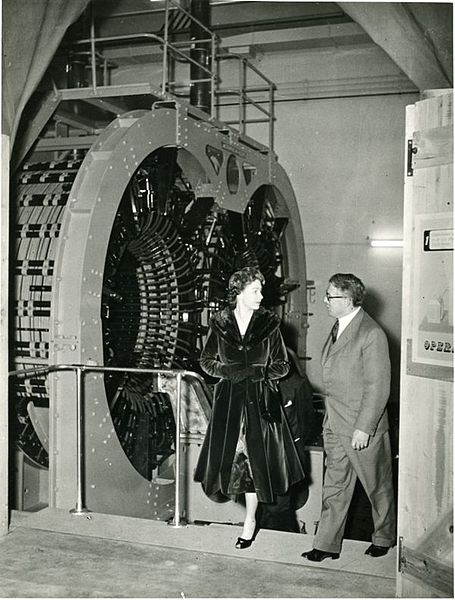
\includegraphics[width = 0.75\linewidth]{./1_Introduction/queen_at_zeta.jpg}
    \label{fig:Queen_at_ZETA}
    \caption[Queen Elizabeth II at the ZETA experiment]{Queen Elizabeth II of Canada and assorted other places, vising ZETA during it's construction in 1957. Photograph by UKAEA}
\end{figure}%

The story of the RFP starts with the Zero Energy Thermonuclear Assembly (ZETA).
Initially built as an extension of the now abandoned toroidal pinch confinement
concept, ZETA was one of the leading fusion experiment of its time, often know
for making and later retracting the first claim of observation of fusion
neutrons, for a time galvanizing world interesting in the imminent arrival of
unlimited energy via fusion. Alas, the claim was made in haste. But persistence
and hard work eventually let scientists at ZETA to discover the spontaneous
reversal of the magnetic field associated with the most stable (quiescent)
period of ZETA's plasmas \cite{Butt_IAEA66,Robinson_IAEA69}. This phenomenon
was explained by J. Taylor in 1974 as a naturally result from the relaxation of
the magnetic topology towards lower energy state \cite{Taylor74}. These were
the foundational documents of the RFP.

\begin{align}\label{eqn:helicity}
	K \equiv \int_{V} \vec{A} \cdot \vec{B} d\tau
\end{align}

Specifically, Taylor posited that in a toroidal plasma of finite resistivity
constrained by a perfectly conducting shell, the magnetic helicity $K$ is
conserved (eqn. \ref{eqn:helicity}). With this constraint, the plasma relaxes
toward a state of minimum magnetic energy characterized by eqn.
\ref{eqn:min_energy_condition}, where $\mu \varpropto K/ \Psi ^2$, is a
constant unrelated to permeability . 

\begin{align}\label{eqn:min_energy_condition}
    \nabla \times \vec{B} = \mu \vec{B}
\end{align}

In cylindrical approximation, the solution to equation
\ref{eqn:min_energy_condition} are Bessel functions (eqn.
\ref{eqn:rfp_solution}) where $B_Z$ reverses in the edge if the plasma current
is high compared to toroidal flux \cite{Taylor74}.

\begin{align}\label{eqn:rfp_solution}
B_z &= B_0J_0(\mu r)\\
B_\theta &= B_0 J_1(\mu r)\\
B_r & = 0
\end{align}

The magnetic topology of atypical RFP is shown in figure
\ref{fig:RFP_geometry}. The relatively low $B_t$ means the RFP have several
advantages over the Tokamak. In the tokamaks, powerful toroidal field coils (TF
coils) are used to generate toroidal flux and keep the safety factor q is kept
above 1 in order to stabilize the plasma. This leads to limits on the toroidal
plasma current depending on the the available coil generated toroidal flux.
This in turns is limited by engineering constrains in terms of magnetic coil
construction. The reversed field pinch avoids these constrains, and
consequently can be constructed with much simpler and cheaper TF coil
arrangements, as well as being more easily reach very high current levels to
take advantage of large Ohmic heating, possibly to ignition levels.

\begin{figure}[!htb]
	\centering
	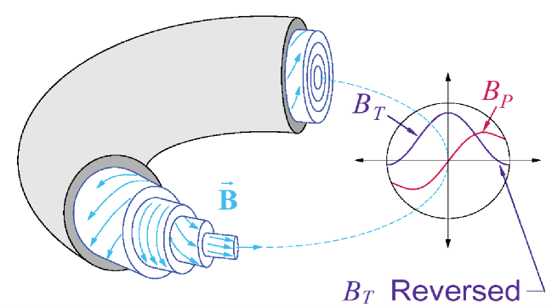
\includegraphics[width = 1.\linewidth]{./1_Introduction/RFP_mag_geometry.png}
	\label{fig:RFP_geometry}
	\caption[RFP magnetic topology]{Illustration of the RFP topology. The most distinct features of the RFP is the similar magnitudes of $B_t$ vs. $B_p$, as well as the fact that $B_p$ reverses direction near the edge.}
\end{figure}%

However, the magnetic topology also poses challenges to the RFP's confinement
characteristics. Taylor noted that the relaxation of the magnetic field is made
possible by the finite resistivity, but did not speculate on the 'method' of
relaxation. Experiments have shown that the relaxation occurs via resistive
tearing mode instabilities which poses a challenge to RFP confinement
characteristics.

\begin{figure}
	\centering
    \label{fig:q_profile}
    
    \caption[Example RPF q profile]{q profile typical of the plasmas studies in this work. Note the closely space resonant surfaces.}

\end{figure}

\section{Tearing modes, it's suppression via PPCD, and improved confinement}
\begin{figure}[!htb]
	\centering
	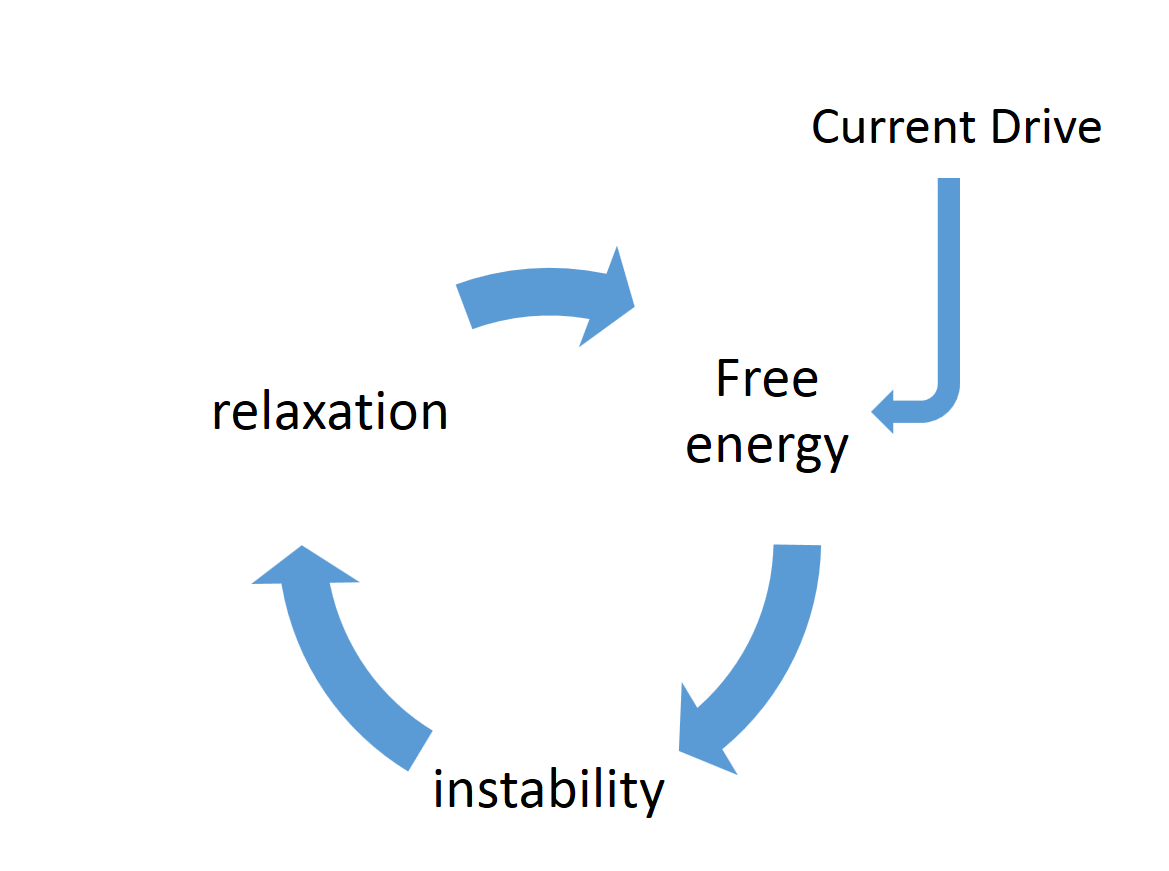
\includegraphics[width = .6\linewidth]{./1_Introduction/the_sawtooth_cycle.PNG}
	\label{fig:sawtooth_cycle}
	\caption[The sawtooth cycle]{The sawtooth cycle that dominates standard RFP plasmas. Improving RFP confinement involves the suppression of this cycle. The PPCD approach involves the suppression of the tearing mode instabilities while inductively driving the plasma current profile relaxation.}
\end{figure}%

The finite resistivity of the plasma allows for the reconnection of the
magnetic field lines and the formation of magnetic islands through tearing mode
instabilities. Tearing modes are unstable at magnetic resonant surfaces where
the safety factor $q \equiv \frac{rB_T}{R_0B_p}$ is a rational number, ie $q =
\frac{m}{n}$ where m and n are integers. The location of these unstable regions
form 'resonant' surfaces that are typically labeled by their m and n numbers.
The RFP have q significantly lower than 1 everywhere, and further decreases
monotonously towards the edge where it will cross 0. An example q profile is
show in figure \ref{fig:q_profile}. This leads to the existence of a large
number of resonant surfaces, especially close to the reversal surface. 

These closely spaced resonant surfaces and the tearing mode instabilities that
they 'host' creates regions of overlapping magnetic islands that turns the
magnetic field stochastic, greatly reducing the confinement characteristics.
Further, the tearing modes in standard RFP enables the violent relaxations
events know as the sawtooth crashes, where the accumulation of free energy in
the form of parallel current ($J_{\parallel}$) gradient will cause a sudden
increase of magnetic reconnection and tearing mode fluctuation. This process
then repeats as the parallel current gradient builds up again in what is know
as the sawtooth cycle (fig \ref{fig:sawtooth_cycle}). Though ion heating is
observed with the sawtooth
crashes\cite{Bodin1980Reversed-field-pinchReserarch}, they greatly disrupts
confinement of particles and limit the RFP's viability as a fusion concept.

\begin{figure}[!htb]
	\centering
	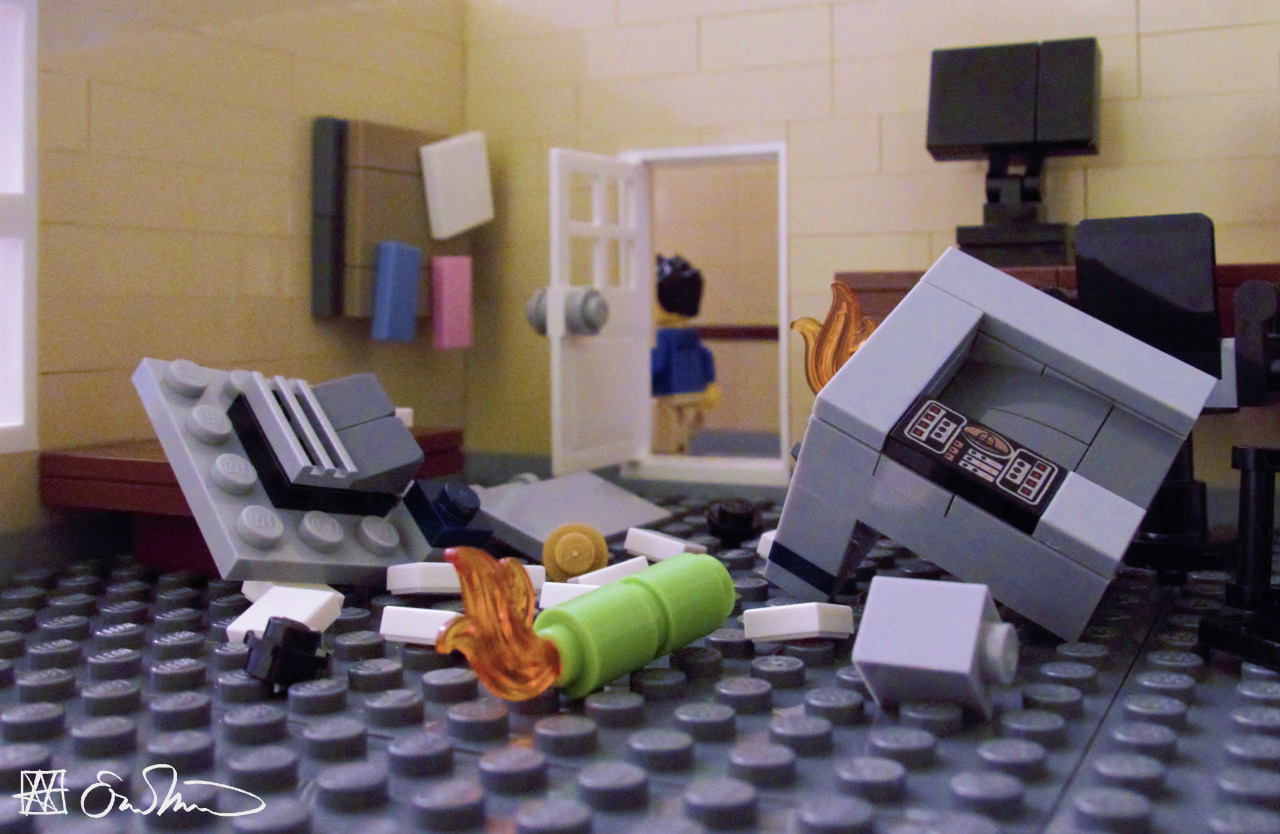
\includegraphics[width = .8\linewidth]{./1_Introduction/violent_relaxation.jpg}
	\label{fig:violet_relaxation}
	\caption[An illustration of violent relaxation]{An artist's impression of a violent relaxation event. By the Lego Grad Student}
\end{figure}%

One very successful way of reducing tearing mode activity and its detrimental
effects on confinement is through the control of $J_{\parallel}$ profile,
thereby reducing the available free energy from it's gradient at the resonant
surfaces\cite{Sarff1995TransportPinch}. On MST, this is done inductively
through a process called Pulsed Parallel Current Drive (PPCD). PPCD drives
parallel currently near the reversal surface (details discussed in section
\ref{sec:MST}), essentially aiding the plasma in reaching itspreferred' state
of with a flat $J_{\parallel}$ profile so it doesn't 'have to' through 'the use
of' sawtooth crashes. Further refinements of this process is also able to
reduce the residual, m = 0 related, magnetic reconnection, achieving
significantly improved confinement for $\geq 10ms$ \cite{Chapman2001}.



\section{Characteristics of PPCD plasma}

PPCD reduces the tearing mode fluctuation levels significantly as shown in
figure \ref{fig:ppcd_fluc}


It is well known that magnetic reconnection such as sawtooth are bad, but are
they cruel? It's a question that have yet to answered in all these years. How
do sawtooth events stack up again the terrible events perpetrated by powerful
men through the ages such as war and famine and worse things. We don't really
know.



They are pretty to look at and stuff. Also Jim Reynolds predicted pinch. Also
significant reduction in fluctuation. Also $T_e$ increase and hot, and have
bursts occasionally, also transport transport transport also stochasticity
decreases, also transient, and some other stuff.


[[Both Santhosh's observation of classical transport but also Reynold's prediction]]


\section{m = 0 bursts in EC and PPCD plasmas}

Bill Young looked at the m = 0 in EC plasmas because he can't look at sawtooth.
Ring like structure, and what not. Also D. Adams made a post for it, measuring
the ring structure, looks good.


[[Bill Young's stuff will be here, as well whatever he cites.]]


\section{What this thesis is all about}
[[Signposting is important]]



Ion transport is important area of research for several reasons in the context
of fusion confinement geometry. The most basic being that it is ion temperature
that is relevant to the rate of fusion reactions. But in particular, there is
long standing disagreement in the field regarding the mechanism behind the well
known anomalous ion heating associated with sawtooth events. At the same time,
there has been confusion about the existence and magnitude of anomalous heating
during periods of improved confinement achieved through parallel current drive.

The RFP geometry suffers from regular global sawtooth events associated with
tearing mode reconnections. While the violent magnetic fluctuations [[Draw
connections with solar and dynamo stuff]]

[Now draw connections with fusion, confinement and whatnot]
\printbibliography%[title={Section bibliography}]

\end{refsection}

\begin{refsection}
\chapter{Experimental Hardware}

MST is a well diagnosed device and my work has involved a large number of plasma diagnostics both directly and indirectly. In this chapter I give a summary of them, their general capabilities, their limitations, and the method of their incorporation into my work. Particular attention is paid to the Ion Doppler Spectrometer II (IDS-II) as it is the diagnostic I was most involved with in a hands-on fashion.

\section{The Madison Symmetric Torus}\label{sec:MST}
The Madison Symmetric Torus is a reversed field pinch device located in Madison, WI. It was constructed in the 1980s, achieving first plasma in 1988.
\begin{figure}[!htb]
	\centering
	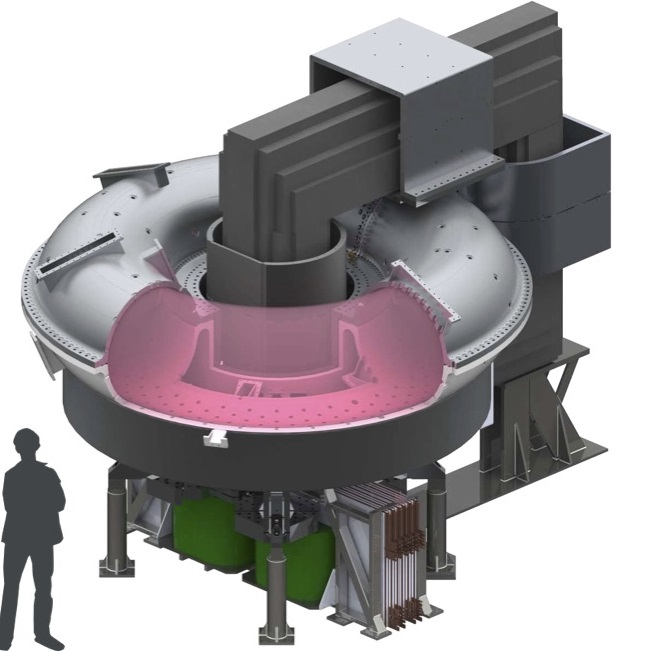
\includegraphics{./2_Experimental_hardware/MST_model_diagram}
	\label{fig:MST_diagram}
	\caption[Diagram of MST]{Diagram of MST. Note the close fitting shell, as well as the holes on the bottom of the vessel that leads to the pumping manifold. It's location will become relevant in section \ref{sec:neutral_dynamics}.}
\end{figure}

I work here!


\begin{figure}[!htb]
	\centering
	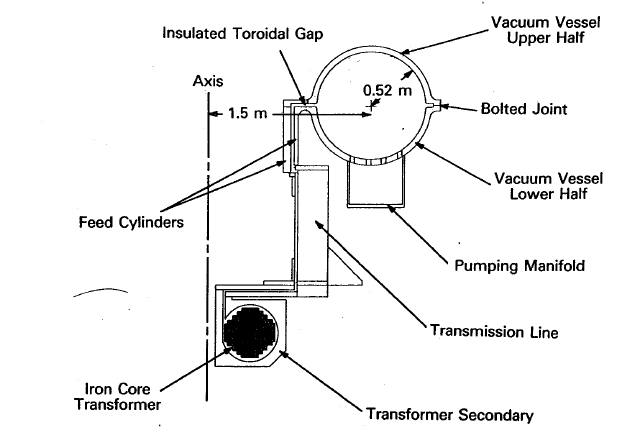
\includegraphics{./2_Experimental_hardware/MST_tor_section.PNG}
	\label{fig:MST_tor_section}
	\caption[Toridal section of MST]{Toroidal section diagram of MST. Note again pumping manifold's location; as well as the transmission line coupling the secondary transformer to the close fitting shell itself. This is what allows the inductive current drive behind PPCD operations. The entire shell is used as a 'TF coil'. (Reproduced from R. Dexter et al. Ref\cite{Dexter100}}
\end{figure}


\section{Magnetic coils, equilibrium reconstruction and MSTfit}
I trust Jay, and didn't look that carefully at any of it\cite{mstfit}.

\section{Far Infrared Interferometer and Polarimeter}
Gets me $n_e$ and $B$.

\section{The $D_{\alpha}$ array}
Gets me neutral information.

\section{The Thompson Scattering Thing}
It's not an interferometer and I don't think it's a spectrometer. So it's just a thing right now.



\section{The Ion Doppler Spectrometer II and Charge Exchange Spectrometry}
Gets me $T_{impurities}$

\printbibliography
\end{refsection}
\chapter{Ion Classical Transport Model Structure and Design}

\section{Why 1-D classical transport?}
Because it's easy. Also $q^2/\epsilon^{3/2} < 0.2$ everywhere, see figure that I have yet to make.

\section{Inputs and assumptions}
Mostly from the diagnostics mentioned in the previous chapter.

\subsection{Ensembling of diagnostic inputs}

\subsection{Geometry}

\subsection{Boundary conditions}

\subsection{Initial conditions}

\subsection{Impurity density and transport}

\subsection{Duel time scale code implementation}

\section{Ion transport terms and their implementation}
Two time scales, based on MSTfit

\subsection{Ion electron equilibration}

\subsection{Classical collisional transport}

\subsection{Neutral "transport": charge exchange loss and electron impact ionization}

\subsection{Flow heating}




\chapter{Core Ion Thermal Transport Results}

\section{Neutral dynamics in MST and it's impact on ion thermal transport}\label{sec:neutral_dynamics}

\section{Pinch observed in the Reverse Field Pinch}
%\section{Observations of inward pinch flow associated with $\vec{E}\times\vec{B}$ drift and it's effect on ion thermal transport}

\section{Comparison of the model results with measurement}

\section{Model predictions for future devices}
\chapter{Edge impurity ion heating associated with m = 0 activity in PPCD}

\section{m = 0 burst activity in PPCD, its identification and its magnetic characteristics}

\section{Observation of impurity heating associated with the m = 0 activities.}

\section{Evidence of Alfv\'enic ion cyclotron heating as the cause of heating observed.}

\section{Classical ion thermal model results of m = 0}
\begin{refsection}


\chapter{Conclusions and remarks}

\section{Summary of results}

A modeling approach is used to characterize ion thermal transport in improved confinement, reduced tearing (PPCD) plasmas in MST. The forward model is constructed in 1-D approximation and includes classical transport physics, charge exchange and particle flow. The model uses a range of diagnostic inputs to provide the plasma profiles (of $T_e$, $n_e$,$n_D$ as well as reconstructed magnetic) to predict $T_i$ evolution from an initial condition. This model is compared to measurement and found to be sufficient in predicting the core temperature evolution, but needed an \adhoc heating source localized in the gradient region to match observations. Additional thermal transport is not required to match measurements. The model includes the calculation of electron-ion equilibration, classical conduction, charge exchange loss, and flow related heating (including compression and convective heat flow). The model is applied to an ensemble of selected 500kA PPCD shots in MST, and it's temperature predictions are compared to measurements of $T_{C^{6+}}$ as a proxy of $T_i$.

The neutral dynamics is found to be important in constructing and analyzing the model. A physics based Monte Carlo simulation is used to calculate the neutral density and charge exchange loss, especially in the core. The simulations show that the core neutrals are 'warm' ($\approx 0.6-0.8 T_i$) and the charge exchange loss profile is hollow. Further, a portion of the energy lost to the neutrals is recovered via subsequent re-ionization. This simulation also provides the ionization source rate profile, which when combined with density measurements show that an inward particle flux in the core is necessary to account for the core density rise early in PPCD. Comparison is made with estimates of \ecb flux in PPCD and found to be a match. The compression effect of this flux is incorporated into the model, as well as the effect of the edge particle outflow. 

%Mark's email comments
%Make sure to list all of the unique things that you can point to which you did in your conclusion chapter. Keep in mind that you have done the most thorough analysis of ion heat transport in PPCD plasmas to date. You’ve done the most thorough analysis of neutral density profile evolution during PPCD which informs not only your ion power balance work, but has also been important in predicting charge state distributions of highly charge ions (like Aluminum) for predicting x-ray emission spectra (Patrick & Lisa’s work for the ME-SXR model and now the LLNL x-ray calorimeter). You’ve shown that any heating beyond classical mechanisms that you’ve called out in your model are edge localized. Your analysis of the m=0 burst activity also suggests that burst heating of the impurities may follow the same type of collisional equilibration with the deuterium that describes the ion heating due to magnetic reconnection present during edge-localized tearing mode excitation in standard plasmas.
%---

An \adhoc heating term is added to the model to match observations. The needed \adhoc term is located near the edge in the gradient region

The model's ion confinement time is found to be , and the largest loss mechanisms are found to be associated with particle loss out of the plasma, with charge exchange a near second. 

The phenomenon of impurity heating associated with m = 0 bursts in PPCD is investigated and found to have interesting properties such as edge locality, (near) simultaneous heating regardless of toroidal or radial location (except where there is no heating), and a faster than expected equilibration time. However, there are still many unclear aspects that surrounds this phenomenon that needs further investigation to clear up. 


This works presents the most thorough accounting for ion thermal transport in PPCD plasmas, and 



\section{Future work}
A more detailed assessment of turbulent heating mechanisms available 
Rutherford scattering measurements of D+ temperature, especially during the 
Direct measurements of neutral temperature. 


\printbibliography
\end{refsection}

% \include{related/related}

%% etc, etc.

%% Do you have appendices?  If so, add them here, just like chapters.
% \begin{appendices}
% \include{backmatter/appendix1}
% \end{appendices}



%% McBride is a very nice style (some version is included in this distribution)
%\bibliographystyle{unsrt}


%% Want an index?  Neither did I.
%\printindex

\end{document}
